\section{Flow\-Shop\-Objective\-Vector\-Traits Class Reference}
\label{classFlowShopObjectiveVectorTraits}\index{FlowShopObjectiveVectorTraits@{FlowShopObjectiveVectorTraits}}
Definition of the objective vector traits for multi-objective flow-shop problems.  


{\tt \#include $<$Flow\-Shop\-Objective\-Vector\-Traits.h$>$}

Inheritance diagram for Flow\-Shop\-Objective\-Vector\-Traits::\begin{figure}[H]
\begin{center}
\leavevmode
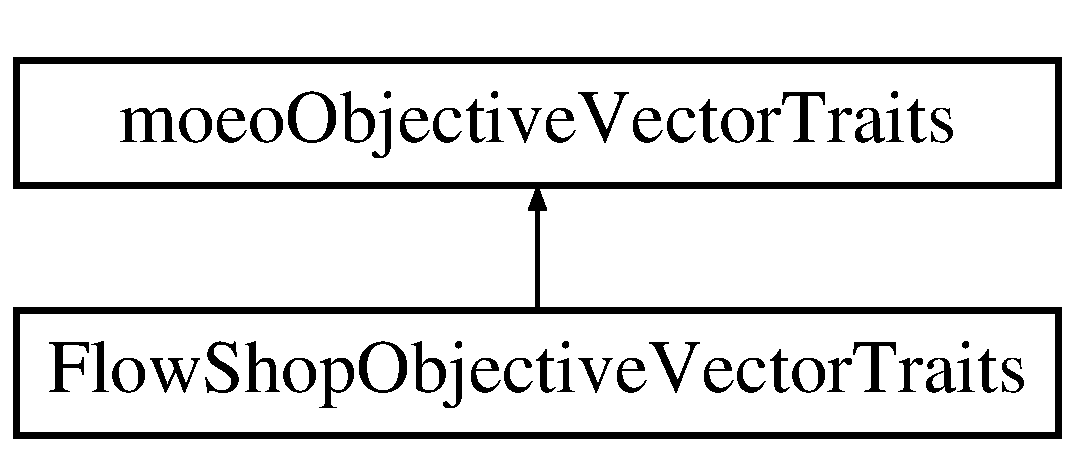
\includegraphics[height=2cm]{classFlowShopObjectiveVectorTraits}
\end{center}
\end{figure}
\subsection*{Static Public Member Functions}
\begin{CompactItemize}
\item 
static bool \bf{minimizing} (int \_\-i)
\begin{CompactList}\small\item\em Returns true if the \_\-ith objective have to be minimzed. \item\end{CompactList}\item 
static bool \bf{maximizing} (int \_\-i)
\begin{CompactList}\small\item\em Returns true if the \_\-ith objective have to be maximzed. \item\end{CompactList}\item 
static unsigned int \bf{n\-Objectives} ()\label{classFlowShopObjectiveVectorTraits_76ebe7639b502980bc683ab404b69c10}

\begin{CompactList}\small\item\em Returns the number of objectives. \item\end{CompactList}\end{CompactItemize}


\subsection{Detailed Description}
Definition of the objective vector traits for multi-objective flow-shop problems. 



Definition at line 46 of file Flow\-Shop\-Objective\-Vector\-Traits.h.

\subsection{Member Function Documentation}
\index{FlowShopObjectiveVectorTraits@{Flow\-Shop\-Objective\-Vector\-Traits}!minimizing@{minimizing}}
\index{minimizing@{minimizing}!FlowShopObjectiveVectorTraits@{Flow\-Shop\-Objective\-Vector\-Traits}}
\subsubsection{\setlength{\rightskip}{0pt plus 5cm}bool Flow\-Shop\-Objective\-Vector\-Traits::minimizing (int {\em \_\-i})\hspace{0.3cm}{\tt  [static]}}\label{classFlowShopObjectiveVectorTraits_e1a0f5be1782b9f9ce08128a404a1fa8}


Returns true if the \_\-ith objective have to be minimzed. 

\begin{Desc}
\item[Parameters:]
\begin{description}
\item[{\em \_\-i}]index of the objective \end{description}
\end{Desc}


Definition at line 41 of file Flow\-Shop\-Objective\-Vector\-Traits.cpp.\index{FlowShopObjectiveVectorTraits@{Flow\-Shop\-Objective\-Vector\-Traits}!maximizing@{maximizing}}
\index{maximizing@{maximizing}!FlowShopObjectiveVectorTraits@{Flow\-Shop\-Objective\-Vector\-Traits}}
\subsubsection{\setlength{\rightskip}{0pt plus 5cm}bool Flow\-Shop\-Objective\-Vector\-Traits::maximizing (int {\em \_\-i})\hspace{0.3cm}{\tt  [static]}}\label{classFlowShopObjectiveVectorTraits_229fbb4cc19d289637891c1b49f3eaba}


Returns true if the \_\-ith objective have to be maximzed. 

\begin{Desc}
\item[Parameters:]
\begin{description}
\item[{\em \_\-i}]index of the objective \end{description}
\end{Desc}


Definition at line 47 of file Flow\-Shop\-Objective\-Vector\-Traits.cpp.

The documentation for this class was generated from the following files:\begin{CompactItemize}
\item 
Flow\-Shop\-Objective\-Vector\-Traits.h\item 
Flow\-Shop\-Objective\-Vector\-Traits.cpp\end{CompactItemize}
